\documentclass[12pt, a4paper]{article}

% ── Packages ──────────────────────────────────────────────────────
\usepackage[utf8]{inputenc}
\usepackage[T1]{fontenc}
\usepackage{amsmath, amssymb, amsthm}
\usepackage{mathtools}
\usepackage{enumitem}
\usepackage{tikz}
\usetikzlibrary{calc, positioning, arrows.meta, fit, patterns, decorations.pathreplacing}
\usepackage{geometry}
\geometry{margin=2.4cm}
\usepackage{xcolor}
\usepackage{tcolorbox}
\tcbuselibrary{theorems, skins, breakable}
\usepackage{booktabs}
\usepackage{hyperref}
\hypersetup{colorlinks=true, linkcolor=blue!60!black, urlcolor=blue!60!black}

\setlength{\parindent}{0pt}
\setlength{\parskip}{6pt}

% ── Colours ───────────────────────────────────────────────────────
\definecolor{setA}{RGB}{66, 133, 244}   % blue
\definecolor{setB}{RGB}{234, 67, 53}    % red
\definecolor{setC}{RGB}{251, 188, 4}    % yellow
\definecolor{theoryBg}{RGB}{232, 245, 253}
\definecolor{theoryFrame}{RGB}{66, 133, 244}
\definecolor{stmtBg}{RGB}{255, 243, 224}
\definecolor{stmtFrame}{RGB}{230, 126, 34}
\definecolor{ansBg}{RGB}{232, 250, 232}
\definecolor{ansFrame}{RGB}{39, 174, 96}

% ── Environments ──────────────────────────────────────────────────
\newtcolorbox{theorybox}[1][]{%
  colback=theoryBg, colframe=theoryFrame,
  fonttitle=\bfseries, title={\small Theory Recap: #1},
  breakable, enhanced, arc=2mm,
  left=5pt, right=5pt, top=5pt, bottom=5pt
}

\newtcolorbox{problembox}{%
  colback=stmtBg, colframe=stmtFrame,
  fonttitle=\bfseries, title={\small Problem Statement},
  breakable, enhanced, arc=2mm,
  left=5pt, right=5pt, top=5pt, bottom=5pt
}

\newtcolorbox{answerbox}{%
  colback=ansBg, colframe=ansFrame,
  arc=2mm, left=5pt, right=5pt, top=3pt, bottom=3pt
}

\newcommand{\Z}{\mathbb{Z}}
\newcommand{\R}{\mathbb{R}}
\newcommand{\N}{\mathbb{N}}
\newcommand{\powset}[1]{2^{#1}}
\newcommand{\comp}[1]{\overline{#1}}
\newcommand{\symdiff}{\mathbin{\triangle}}

% ── Title ─────────────────────────────────────────────────────────
\title{\textbf{Practice 7 --- Partitions \& Inclusion-Exclusion}\\[4pt]
       \large Solutions to Selected Problems\\[2pt]
       \normalsize Problems 1, 7, 10, 12}
\author{Discrete Mathematics --- QYSU}
\date{}

\begin{document}
\maketitle
\tableofcontents
\newpage

% ══════════════════════════════════════════════════════════════════
\section{Problem 1 --- Partitions of a 5-Element Set into 3 Classes}
% ══════════════════════════════════════════════════════════════════

\begin{theorybox}[Stirling Numbers of the Second Kind]
The \textbf{Stirling number of the second kind} $S(n,k)$ counts the number
of ways to partition an $n$-element set into exactly $k$ non-empty,
pairwise disjoint subsets (called \emph{classes} or \emph{blocks}).

\medskip
\textbf{Recurrence relation:}
\[
  S(n,k) = S(n-1,\, k-1) \;+\; k \cdot S(n-1,\, k),
  \qquad n \ge 1,\; 1 \le k \le n.
\]

\textbf{Interpretation:}\; Consider element $n$.
\begin{itemize}[nosep]
  \item \emph{$n$ is alone in its own class:}\;
        the remaining $n-1$ elements form $k-1$ classes
        $\;\longrightarrow\; S(n-1,\,k-1)$ ways.
  \item \emph{$n$ joins one of the existing $k$ classes:}\;
        first partition the other $n-1$ elements into $k$ classes
        ($S(n-1,\,k)$ ways), then choose which class $n$ joins ($k$ choices)
        $\;\longrightarrow\; k \cdot S(n-1,\,k)$ ways.
\end{itemize}

\medskip
\textbf{Boundary conditions:}\;
$S(n,1) = 1$,\; $S(n,n) = 1$,\; $S(n,0) = 0$ for $n \ge 1$.

\begin{center}
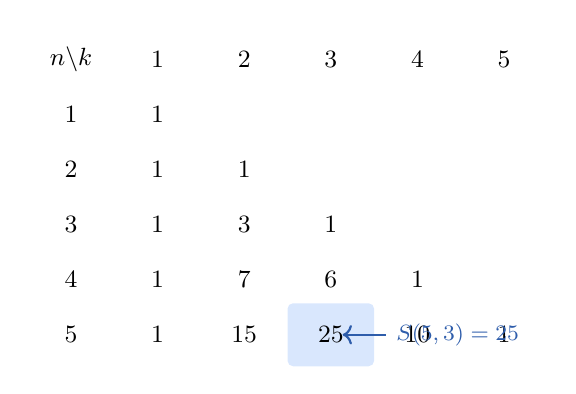
\begin{tikzpicture}[
  cell/.style={minimum width=1.1cm, minimum height=0.8cm, font=\small, anchor=center},
  header/.style={cell, font=\small\bfseries}
]
  % Header row
  \node[header] at (0, 0) {$n \backslash k$};
  \foreach \k [count=\i] in {1,2,3,4,5} {
    \node[header] at (\i*1.1, 0) {$\k$};
  }
  % Data rows
  \foreach \n/\vals [count=\row] in {
    1/{1},
    2/{1,1},
    3/{1,3,1},
    4/{1,7,6,1},
    5/{1,15,25,10,1}%
  } {
    \node[cell, font=\small\bfseries] at (0, -\row*0.7) {$\n$};
    \foreach \v [count=\col] in \vals {
      \ifnum\row=5
        \ifnum\col=3
          \node[cell, fill=setA!20, rounded corners=2pt] at (\col*1.1, -\row*0.7) {$\v$};
        \else
          \node[cell] at (\col*1.1, -\row*0.7) {$\v$};
        \fi
      \else
        \node[cell] at (\col*1.1, -\row*0.7) {$\v$};
      \fi
    }
  }
  % Highlight annotation
  \draw[->, thick, setA!70!black] (3.3+0.7, -3.5) -- (3.3+0.15, -3.5)
    node[right, pos=0, font=\footnotesize, setA!70!black] {$S(5,3)=25$};
\end{tikzpicture}
\end{center}
\end{theorybox}

\begin{problembox}
In how many ways can a $5$-element set be partitioned into $3$ non-empty classes?
\end{problembox}

\subsection*{Solution}

We need the Stirling number $S(5,3)$. Using the recurrence:
\[
  S(5,3) = S(4,2) + 3 \cdot S(4,3).
\]

\textbf{Computing $S(4,2)$:}
\[
  S(4,2) = S(3,1) + 2 \cdot S(3,2) = 1 + 2 \cdot 3 = 7.
\]

\textbf{Computing $S(4,3)$:}
\[
  S(4,3) = S(3,2) + 3 \cdot S(3,3) = 3 + 3 \cdot 1 = 6.
\]

\textbf{Final result:}
\[
  S(5,3) = 7 + 3 \cdot 6 = 7 + 18 = 25.
\]

\textbf{Verification by explicit enumeration.}\;
Let $\{a,b,c,d,e\}$ be our set. A partition into 3 classes must have
type $\{3,1,1\}$ or $\{2,2,1\}$ (the only integer partitions of 5 into 3 parts).

\begin{itemize}[nosep]
  \item \textbf{Type $\{3,1,1\}$:}\;
        Choose the 3-element block: $\binom{5}{3} = 10$ ways.
        The remaining 2 singletons form an unordered pair, giving $1$ arrangement.
        Total: $10$.
  \item \textbf{Type $\{2,2,1\}$:}\;
        Choose the singleton: $\binom{5}{1} = 5$ ways.
        Partition the remaining 4 elements into two pairs:
        $\frac{1}{2!}\binom{4}{2} = 3$ ways (divide by $2!$ since the two pairs
        are unordered).
        Total: $5 \times 3 = 15$.
\end{itemize}

Grand total: $10 + 15 = 25$. \;\checkmark

\begin{answerbox}
\centering $S(5,3) = \boxed{25}$
\end{answerbox}

% ══════════════════════════════════════════════════════════════════
\newpage
\section{Problem 7 --- Divisibility with Inclusion-Exclusion}
% ══════════════════════════════════════════════════════════════════

\begin{theorybox}[Inclusion-Exclusion Principle]
For events (or sets) $A_1, A_2, \ldots, A_m$ in a finite universe:
\[
  \biggl|\,\bigcup_{i=1}^{m} A_i\biggr|
  = \sum_{i} |A_i|
  - \sum_{i<j} |A_i \cap A_j|
  + \sum_{i<j<k} |A_i \cap A_j \cap A_k|
  - \cdots
\]

To count elements that belong to \textbf{none} of $A_1, \ldots, A_m$:
\[
  \bigl|\comp{A_1} \cap \comp{A_2} \cap \cdots \cap \comp{A_m}\bigr|
  = |U| - \biggl|\,\bigcup_{i=1}^{m} A_i\biggr|.
\]

\medskip
\textbf{Divisibility application:}\;
The number of integers in $\{1, 2, \ldots, N\}$ divisible by $d$ is
$\lfloor N/d \rfloor$.
If $\gcd(d_1, d_2) = 1$, then divisibility by both $d_1$ and $d_2$
is the same as divisibility by $d_1 d_2$.

\begin{center}
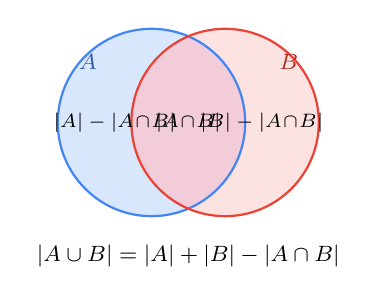
\begin{tikzpicture}[>=Stealth, font=\small, scale=0.85]
  \def\rr{1.4}
  \coordinate (cA) at (-0.55, 0);
  \coordinate (cB) at (0.55, 0);

  % Shade A only
  \begin{scope}
    \clip (cA) circle (\rr);
    \fill[setA!20] (-3,-3) rectangle (3,3);
  \end{scope}
  % Shade B only
  \begin{scope}
    \clip (cB) circle (\rr);
    \fill[setB!15] (-3,-3) rectangle (3,3);
  \end{scope}
  % Overlap
  \begin{scope}
    \clip (cA) circle (\rr);
    \clip (cB) circle (\rr);
    \fill[purple!20] (-3,-3) rectangle (3,3);
  \end{scope}

  \draw[thick, setA] (cA) circle (\rr);
  \draw[thick, setB] (cB) circle (\rr);

  \node[font=\footnotesize\bfseries, setA!70!black] at (-1.5, 0.9) {$A$};
  \node[font=\footnotesize\bfseries, setB!70!black] at (1.5, 0.9) {$B$};

  \node[font=\scriptsize] at (-1.1, 0) {$|A|-|A\!\cap\! B|$};
  \node[font=\scriptsize] at (0, 0) {$|A\!\cap\! B|$};
  \node[font=\scriptsize] at (1.1, 0) {$|B|-|A\!\cap\! B|$};

  \node[font=\footnotesize] at (0, -2.0) {$|A \cup B| = |A| + |B| - |A \cap B|$};
\end{tikzpicture}
\end{center}
\end{theorybox}

\begin{problembox}
How many integers between $1$ and $16500$ are not divisible by $5$
and not divisible by $3$, but \textbf{are} divisible by $11$?
\end{problembox}

\subsection*{Solution}

Let $S$ be the set of integers in $\{1, 2, \ldots, 16500\}$ that are
divisible by $11$. We want to remove from $S$ those elements also
divisible by $3$ or by $5$.

Define:
\begin{align*}
  A &= \{n \in S \mid 3 \mid n\}
      &&\text{(divisible by both 11 and 3, i.e.\ by 33)}, \\
  B &= \{n \in S \mid 5 \mid n\}
      &&\text{(divisible by both 11 and 5, i.e.\ by 55)}.
\end{align*}

We seek $|S| - |A \cup B|$.

\textbf{Step 1: Compute individual counts.}
\[
\renewcommand{\arraystretch}{1.3}
\begin{array}{rclcl}
  |S| &=& \lfloor 16500/11 \rfloor &=& 1500, \\
  |A| &=& \lfloor 16500/33 \rfloor &=& 500, \\
  |B| &=& \lfloor 16500/55 \rfloor &=& 300, \\
  |A \cap B| &=& \lfloor 16500/165 \rfloor &=& 100.
\end{array}
\]
Here $|A \cap B|$ counts integers divisible by $\text{lcm}(33,55) = 165$.

\textbf{Step 2: Apply inclusion-exclusion.}
\[
  |A \cup B| = |A| + |B| - |A \cap B| = 500 + 300 - 100 = 700.
\]

\textbf{Step 3: Subtract.}
\[
  |S \setminus (A \cup B)| = |S| - |A \cup B| = 1500 - 700 = 800.
\]

\begin{center}
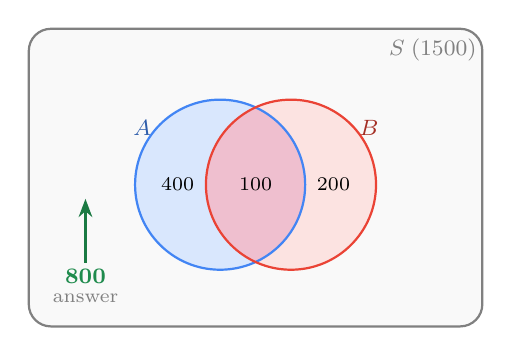
\begin{tikzpicture}[>=Stealth, font=\small, scale=0.9]
  % Universe = S (div by 11)
  \draw[thick, gray, rounded corners=8pt, fill=gray!5]
    (-3.2, -2.0) rectangle (3.2, 2.2);
  \node[gray, font=\footnotesize\bfseries] at (2.5, 1.9) {$S\;(1500)$};

  \def\rr{1.2}
  \coordinate (cA) at (-0.5, 0);
  \coordinate (cB) at (0.5, 0);

  \fill[setA!20] (cA) circle (\rr);
  \fill[setB!15] (cB) circle (\rr);
  \begin{scope}
    \clip (cA) circle (\rr);
    \fill[purple!25] (cB) circle (\rr);
  \end{scope}

  \draw[thick, setA] (cA) circle (\rr);
  \draw[thick, setB] (cB) circle (\rr);

  \node[font=\footnotesize\bfseries, setA!70!black] at (-1.6, 0.8) {$A$};
  \node[font=\footnotesize\bfseries, setB!70!black] at (1.6, 0.8) {$B$};

  \node[font=\scriptsize] at (-1.1, 0) {$400$};
  \node[font=\scriptsize] at (0, 0) {$100$};
  \node[font=\scriptsize] at (1.1, 0) {$200$};

  \node[font=\footnotesize, ansFrame!80!black] at (-2.4, -1.3) {\textbf{800}};
  \draw[->, thick, ansFrame!70!black] (-2.4, -1.1) -- (-2.4, -0.2);
  \node[font=\scriptsize, gray] at (-2.4, -1.6) {answer};
\end{tikzpicture}
\end{center}

\begin{answerbox}
\centering $\boxed{800}$ integers between 1 and 16500 are divisible by 11
but not by 3 and not by 5.
\end{answerbox}

% ══════════════════════════════════════════════════════════════════
\newpage
\section{Problem 10 --- Triangles in a Triangular Grid}
% ══════════════════════════════════════════════════════════════════

\begin{theorybox}[Counting Triangles in a Triangular Grid]
When each side of an equilateral triangle is divided into $n$ equal segments,
connecting the division points with lines parallel to all three sides creates
a \textbf{triangular grid} of side $n$.

\medskip
The grid contains two types of triangles with sides parallel to the original:

\begin{enumerate}[nosep]
  \item \textbf{Upward-pointing} triangles (same orientation as the original)
        of side length $s$ ($1 \le s \le n$):
        \[
          U(n,s) = \frac{(n-s+1)(n-s+2)}{2} = \binom{n-s+2}{2}.
        \]
  \item \textbf{Downward-pointing} triangles (inverted orientation)
        of side length $s$ ($1 \le s \le \lfloor n/2 \rfloor$):
        \[
          D(n,s) = \frac{(n-2s+1)(n-2s+2)}{2} = \binom{n-2s+2}{2}.
        \]
\end{enumerate}

\begin{center}
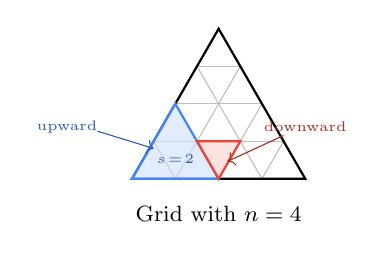
\begin{tikzpicture}[scale=0.55, font=\small]
  % Small grid n=4 for illustration
  \def\n{4}
  % Draw grid lines
  \foreach \i in {0,...,\n} {
    % horizontal-ish lines (parallel to base)
    \draw[gray!50] (\i/2, {\i*sqrt(3)/2}) -- (\n - \i/2, {\i*sqrt(3)/2});
    % left-leaning lines
    \draw[gray!50] (\i, 0) -- (\i/2, {\i*sqrt(3)/2});
    % right-leaning lines
    \draw[gray!50] (\i, 0) -- ({(\n+\i)/2}, {(\n-\i)*sqrt(3)/2});
  }
  % Outer triangle
  \draw[thick] (0,0) -- (\n, 0) -- (\n/2, {\n*sqrt(3)/2}) -- cycle;

  % Highlight an upward triangle of side 2 (blue)
  \fill[setA!25, opacity=0.6] (0,0) -- (2,0) -- (1, {sqrt(3)}) -- cycle;
  \draw[thick, setA] (0,0) -- (2,0) -- (1, {sqrt(3)}) -- cycle;
  \node[font=\tiny, setA!70!black] at (1, 0.45) {$s\!=\!2$};

  % Highlight a downward triangle of side 1 (red)
  \fill[setB!25, opacity=0.6] (1.5, {sqrt(3)/2}) -- (2, 0) -- (2.5, {sqrt(3)/2}) -- cycle;
  \draw[thick, setB] (1.5, {sqrt(3)/2}) -- (2, 0) -- (2.5, {sqrt(3)/2}) -- cycle;

  % Labels
  \node[font=\footnotesize] at (2, -0.8) {Grid with $n=4$};
  \node[font=\tiny, setA!70!black] at (-1.5, 1.2) {upward};
  \draw[->, setA!70!black, thin] (-0.8, 1.1) -- (0.5, 0.7);
  \node[font=\tiny, setB!70!black] at (4.0, 1.2) {downward};
  \draw[->, setB!70!black, thin] (3.5, 1.0) -- (2.2, 0.4);
\end{tikzpicture}
\end{center}
\end{theorybox}

\begin{problembox}
Each side of triangle $ABC$ is divided into $8$ equal segments.
Lines through the division points parallel to the sides create a triangular grid.
How many triangles can be formed with vertices at these grid points
such that their sides are parallel to the sides of $ABC$?
\end{problembox}

\subsection*{Solution}

We have a triangular grid with $n = 8$. We count upward-pointing and
downward-pointing triangles separately.

\textbf{Upward-pointing triangles of side $s$\; ($1 \le s \le 8$):}
\[
  U(8,s) = \frac{(8-s+1)(8-s+2)}{2} = \binom{10-s}{2}.
\]

\begin{center}
\renewcommand{\arraystretch}{1.3}
\begin{tabular}{c|cccccccc|c}
\toprule
$s$ & 1 & 2 & 3 & 4 & 5 & 6 & 7 & 8 & Total \\
\midrule
$U(8,s)$ & 36 & 28 & 21 & 15 & 10 & 6 & 3 & 1 & \textbf{120} \\
\bottomrule
\end{tabular}
\end{center}

\[
  \sum_{s=1}^{8} U(8,s) = 36 + 28 + 21 + 15 + 10 + 6 + 3 + 1 = 120.
\]

\textbf{Downward-pointing triangles of side $s$\;
($1 \le s \le \lfloor 8/2 \rfloor = 4$):}
\[
  D(8,s) = \frac{(8-2s+1)(8-2s+2)}{2} = \binom{10-2s}{2}.
\]

\begin{center}
\renewcommand{\arraystretch}{1.3}
\begin{tabular}{c|cccc|c}
\toprule
$s$ & 1 & 2 & 3 & 4 & Total \\
\midrule
$D(8,s)$ & 28 & 15 & 6 & 1 & \textbf{50} \\
\bottomrule
\end{tabular}
\end{center}

\[
  \sum_{s=1}^{4} D(8,s) = 28 + 15 + 6 + 1 = 50.
\]

\textbf{Grand total:}
\[
  120 + 50 = 170.
\]

\begin{center}
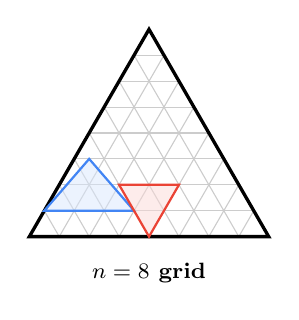
\begin{tikzpicture}[scale=0.38, font=\small]
  % Draw the n=8 grid
  \def\n{8}
  \foreach \i in {0,...,\n} {
    \draw[gray!40] (\i/2, {\i*sqrt(3)/2}) -- (\n - \i/2, {\i*sqrt(3)/2});
    \draw[gray!40] (\i, 0) -- (\i/2, {\i*sqrt(3)/2});
    \draw[gray!40] (\i, 0) -- ({(\n+\i)/2}, {(\n-\i)*sqrt(3)/2});
  }
  \draw[very thick] (0,0) -- (\n, 0) -- (\n/2, {\n*sqrt(3)/2}) -- cycle;

  % Example upward triangle of side 3 (blue)
  \fill[setA!20, opacity=0.5] (0.5, {sqrt(3)/2}) -- (3.5, {sqrt(3)/2})
    -- (2, {3*sqrt(3)/2}) -- cycle;
  \draw[thick, setA] (0.5, {sqrt(3)/2}) -- (3.5, {sqrt(3)/2})
    -- (2, {3*sqrt(3)/2}) -- cycle;

  % Example downward triangle of side 2 (red)
  \fill[setB!20, opacity=0.5] (3, {2*sqrt(3)/2}) -- (5, {2*sqrt(3)/2})
    -- (4, {0*sqrt(3)/2+0}) -- cycle;
  \draw[thick, setB] (3, {2*sqrt(3)/2}) -- (5, {2*sqrt(3)/2})
    -- (4, 0) -- cycle;

  \node[font=\footnotesize\bfseries] at (4, -1.2) {$n = 8$ grid};
\end{tikzpicture}
\end{center}

\begin{answerbox}
\centering The total number of triangles with sides parallel to $ABC$ is
$\boxed{170}$\; (120 upward $+$ 50 downward).
\end{answerbox}

% ══════════════════════════════════════════════════════════════════
\newpage
\section{Problem 12 --- Bounded Integer Solutions via Inclusion-Exclusion}
% ══════════════════════════════════════════════════════════════════

\begin{theorybox}[Counting Integer Solutions with Upper Bounds]
To count non-negative integer solutions to $y_1 + y_2 + \cdots + y_r = n$
with upper bounds $y_i \le u_i$:

\begin{enumerate}[nosep]
  \item \textbf{Without upper bounds:}\;
        The number of solutions is $\binom{n+r-1}{r-1}$ (stars and bars).
  \item \textbf{Subtract violations} using inclusion-exclusion.
        Let $A_i$ be the set of solutions where $y_i > u_i$.
        Substituting $z_i = y_i - (u_i + 1) \ge 0$, the count $|A_i|$
        becomes the unrestricted count with a reduced sum.
  \item \textbf{Intersections:}\;
        $|A_i \cap A_j|$ substitutes both $z_i = y_i - (u_i+1)$
        and $z_j = y_j - (u_j+1)$.
        If the remaining sum is negative, there are $0$ solutions.
\end{enumerate}

\medskip
\textbf{Formula:}
\[
  \text{answer} = \sum_{S \subseteq \{1,\ldots,r\}} (-1)^{|S|}
  \binom{n - \sum_{i \in S}(u_i+1) + r - 1}{r-1},
\]
where terms with a negative top entry in the binomial coefficient are $0$.
\end{theorybox}

\begin{problembox}
Find the number of integer solutions to
\[
  x_1 + x_2 + x_3 = 40, \qquad
  4 \le x_1 \le 15, \quad
  9 \le x_2 \le 18, \quad
  5 \le x_3 \le 16.
\]
\end{problembox}

\subsection*{Solution}

\textbf{Step 1: Shift variables to remove lower bounds.}

Set $y_1 = x_1 - 4$,\; $y_2 = x_2 - 9$,\; $y_3 = x_3 - 5$.
Then:
\[
  y_1 + y_2 + y_3 = 40 - 4 - 9 - 5 = 22,
\]
with bounds $0 \le y_1 \le 11$,\; $0 \le y_2 \le 9$,\; $0 \le y_3 \le 11$.

\textbf{Step 2: Count without upper bounds.}

Without upper bounds, the number of non-negative integer solutions to
$y_1 + y_2 + y_3 = 22$ is:
\[
  \binom{22 + 2}{2} = \binom{24}{2} = 276.
\]

\textbf{Step 3: Define violation sets and apply inclusion-exclusion.}

Let $A_i$ be the set of solutions where $y_i$ exceeds its upper bound:
\begin{align*}
  A_1 &:\; y_1 \ge 12. \quad
        \text{Set } z_1 = y_1 - 12 \ge 0;\;
        z_1 + y_2 + y_3 = 10.
  &\quad |A_1| &= \binom{12}{2} = 66. \\
  A_2 &:\; y_2 \ge 10. \quad
        \text{Set } z_2 = y_2 - 10 \ge 0;\;
        y_1 + z_2 + y_3 = 12.
  &\quad |A_2| &= \binom{14}{2} = 91. \\
  A_3 &:\; y_3 \ge 12. \quad
        \text{Set } z_3 = y_3 - 12 \ge 0;\;
        y_1 + y_2 + z_3 = 10.
  &\quad |A_3| &= \binom{12}{2} = 66.
\end{align*}

\textbf{Step 4: Pairwise intersections.}
\begin{align*}
  A_1 \cap A_2 &:\; y_1 \ge 12,\; y_2 \ge 10.
        \quad \text{Remaining sum: } 22 - 12 - 10 = 0.
  &\quad |A_1 \cap A_2| &= \binom{2}{2} = 1. \\
  A_1 \cap A_3 &:\; y_1 \ge 12,\; y_3 \ge 12.
        \quad \text{Remaining sum: } 22 - 12 - 12 = -2 < 0.
  &\quad |A_1 \cap A_3| &= 0. \\
  A_2 \cap A_3 &:\; y_2 \ge 10,\; y_3 \ge 12.
        \quad \text{Remaining sum: } 22 - 10 - 12 = 0.
  &\quad |A_2 \cap A_3| &= \binom{2}{2} = 1.
\end{align*}

\textbf{Step 5: Triple intersection.}
\[
  A_1 \cap A_2 \cap A_3:\; y_1 \ge 12,\; y_2 \ge 10,\; y_3 \ge 12.
  \quad \text{Sum } \ge 34 > 22. \quad |A_1 \cap A_2 \cap A_3| = 0.
\]

\textbf{Step 6: Combine by inclusion-exclusion.}
\begin{align*}
  |A_1 \cup A_2 \cup A_3|
  &= (66 + 91 + 66) - (1 + 0 + 1) + 0 \\
  &= 223 - 2 = 221.
\end{align*}

\textbf{Final count:}
\[
  276 - 221 = 55.
\]

\begin{center}
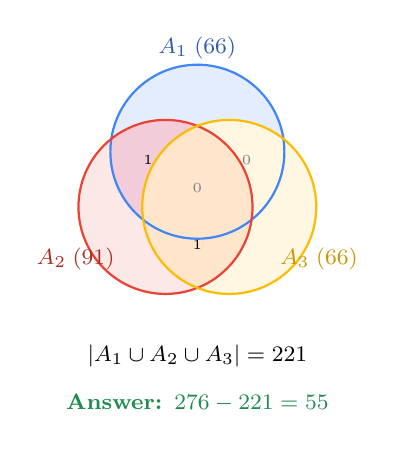
\begin{tikzpicture}[>=Stealth, font=\small, scale=0.85]
  \def\rr{1.3}
  \coordinate (cA) at (90:0.55);
  \coordinate (cB) at (210:0.55);
  \coordinate (cC) at (330:0.55);

  \fill[setA!15] (cA) circle (\rr);
  \fill[setB!12] (cB) circle (\rr);
  \fill[setC!12] (cC) circle (\rr);

  % Pairwise overlaps
  \begin{scope}
    \clip (cA) circle (\rr);
    \fill[purple!20] (cB) circle (\rr);
  \end{scope}
  \begin{scope}
    \clip (cB) circle (\rr);
    \fill[orange!20] (cC) circle (\rr);
  \end{scope}

  \draw[thick, setA] (cA) circle (\rr);
  \draw[thick, setB] (cB) circle (\rr);
  \draw[thick, setC] (cC) circle (\rr);

  \node[font=\footnotesize\bfseries, setA!70!black] at (90:2.1) {$A_1\;(66)$};
  \node[font=\footnotesize\bfseries, setB!70!black] at (210:2.1) {$A_2\;(91)$};
  \node[font=\footnotesize\bfseries, setC!80!black] at (330:2.1) {$A_3\;(66)$};

  \node[font=\tiny] at (150:0.85) {$1$};
  \node[font=\tiny, gray] at (30:0.85) {$0$};
  \node[font=\tiny] at (270:0.85) {$1$};
  \node[font=\tiny, gray] at (0:0) {$0$};

  \node[font=\footnotesize] at (0, -2.5)
    {$|A_1 \cup A_2 \cup A_3| = 221$};
  \node[font=\footnotesize\bfseries, ansFrame!80!black] at (0, -3.2)
    {Answer: $276 - 221 = 55$};
\end{tikzpicture}
\end{center}

\begin{answerbox}
\centering The number of integer solutions is $\boxed{55}$.
\end{answerbox}

\end{document}
